% !TeX root = ../Book3.tex
\begin{tikzpicture}[x=3.1cm,y=3.7cm,>=stealth]
	\draw[->] (0,0)--(2.15,0) node[right] {\(R\)};
	\draw[->] (0,0)--(0,1.12) node[above] {\(E(u_\varepsilon;D_R)/(4\pi)\)};
	\draw[densely dotted,gray] (0,1)--(2,1);
	\node[left] at (0,1) {\(1\)};
	\draw[densely dotted,gray] (0,.5)--(1,.5);
	\node[left] at (0,.5) {\(\tfrac12\)};
	\draw[very thick,blue!75!black,domain=0:2,samples=101]
		plot (\x,{\x*\x/(.0625+\x*\x)});
	\draw[thick,red!75!black,dashed,domain=0:2,samples=101]
		plot (\x,{\x*\x/(1+\x*\x)});
	\draw[densely dotted,blue!75!black] (.25,0)--(.25,.5);
	\draw[densely dotted,red!75!black] (1,0)--(1,.5);
	\fill[blue!75!black] (.25,.5) circle (1.5pt);
	\fill[red!75!black] (1,.5) circle (1.5pt);
	\node[below] at (.25,0) {\(\tfrac14\)};
	\node[below] at (1,0) {\(1\)};
	\node[below] at (2,0) {\(2\)};
	\node[below left] at (0,0) {\(0\)};
	\draw[very thick,blue!75!black] (1.22,.35)--(1.4,.35);
	\node[right] at (1.42,.35) {\(\varepsilon=\tfrac14\)};
	\draw[thick,red!75!black,dashed] (1.22,.18)--(1.4,.18);
	\node[right] at (1.42,.18) {\(\varepsilon=1\)};
\end{tikzpicture}
